\documentclass[aspectratio=169, table]{beamer}


%\usepackage[beamertheme=./praditatheme]{Pradita}

\usetheme{Pradita}

\subtitle{IF231303-Software Architecture}
\title{\huge Chapter-9:\\Mikrokernel/Plugin\\Architecture}
\date[Serial]{\scriptsize {PRU/SPMI/FR-BM-18/0222}}
\author[Pradita]{\small {\textbf{Paris Matio, Brayan Elmer P, Richard Haryono\\ Alfa Yohannis}}}

\begin{document}


    \begin{frame}[plain]
        \maketitle
    \end{frame}

    % Slide 1: Pendahuluan
    \begin{frame}{Pendahuluan}
        \begin{itemize}
            \item Arsitektur Microkernel/Plugin adalah pola desain perangkat lunak yang membagi sistem operasi (OS) menjadi komponen-komponen kecil dan modular.
            \item Presentasi ini membahas definisi, arsitektur, proses, keuntungan, kerugian, dan contoh-contoh Arsitektur Microkernel/Plugin dalam sistem perangkat lunak.
        \end{itemize}
    \end{frame}

    % Slide 2: Definisi
    \begin{frame}{Definisi}
        \begin{itemize}
            \item Arsitektur Microkernel/Plugin adalah pola arsitektural di mana fungsionalitas inti dari sistem, yang dikenal sebagai mikrokernel, dijaga seminimal mungkin.
            \item Fungsionalitas tambahan diimplementasikan sebagai plugin atau modul yang dapat dimuat dan dimuat dari sistem secara dinamis.
        \end{itemize}
    \end{frame}

    % Slide 3: Arsitektur
    \begin{frame}{Arsitektur}
        \begin{itemize}
            \item Dalam Arsitektur Microkernel/Plugin, mikrokernel menyediakan layanan dasar seperti manajemen memori, penjadwalan proses, dan komunikasi antar-proses.
            \item Plugin atau modul memperluas fungsionalitas sistem dengan menyediakan layanan seperti driver perangkat, sistem file, dan protokol jaringan.
        \end{itemize}
    \end{frame}


    \begin{frame}{Mikrokernel dalam Sistem Operasi}
    % \framesubtitle{\hspace{1cm}}
    \begin{columns}
        \begin{column}{0.5\textwidth}
            \begin{center}
                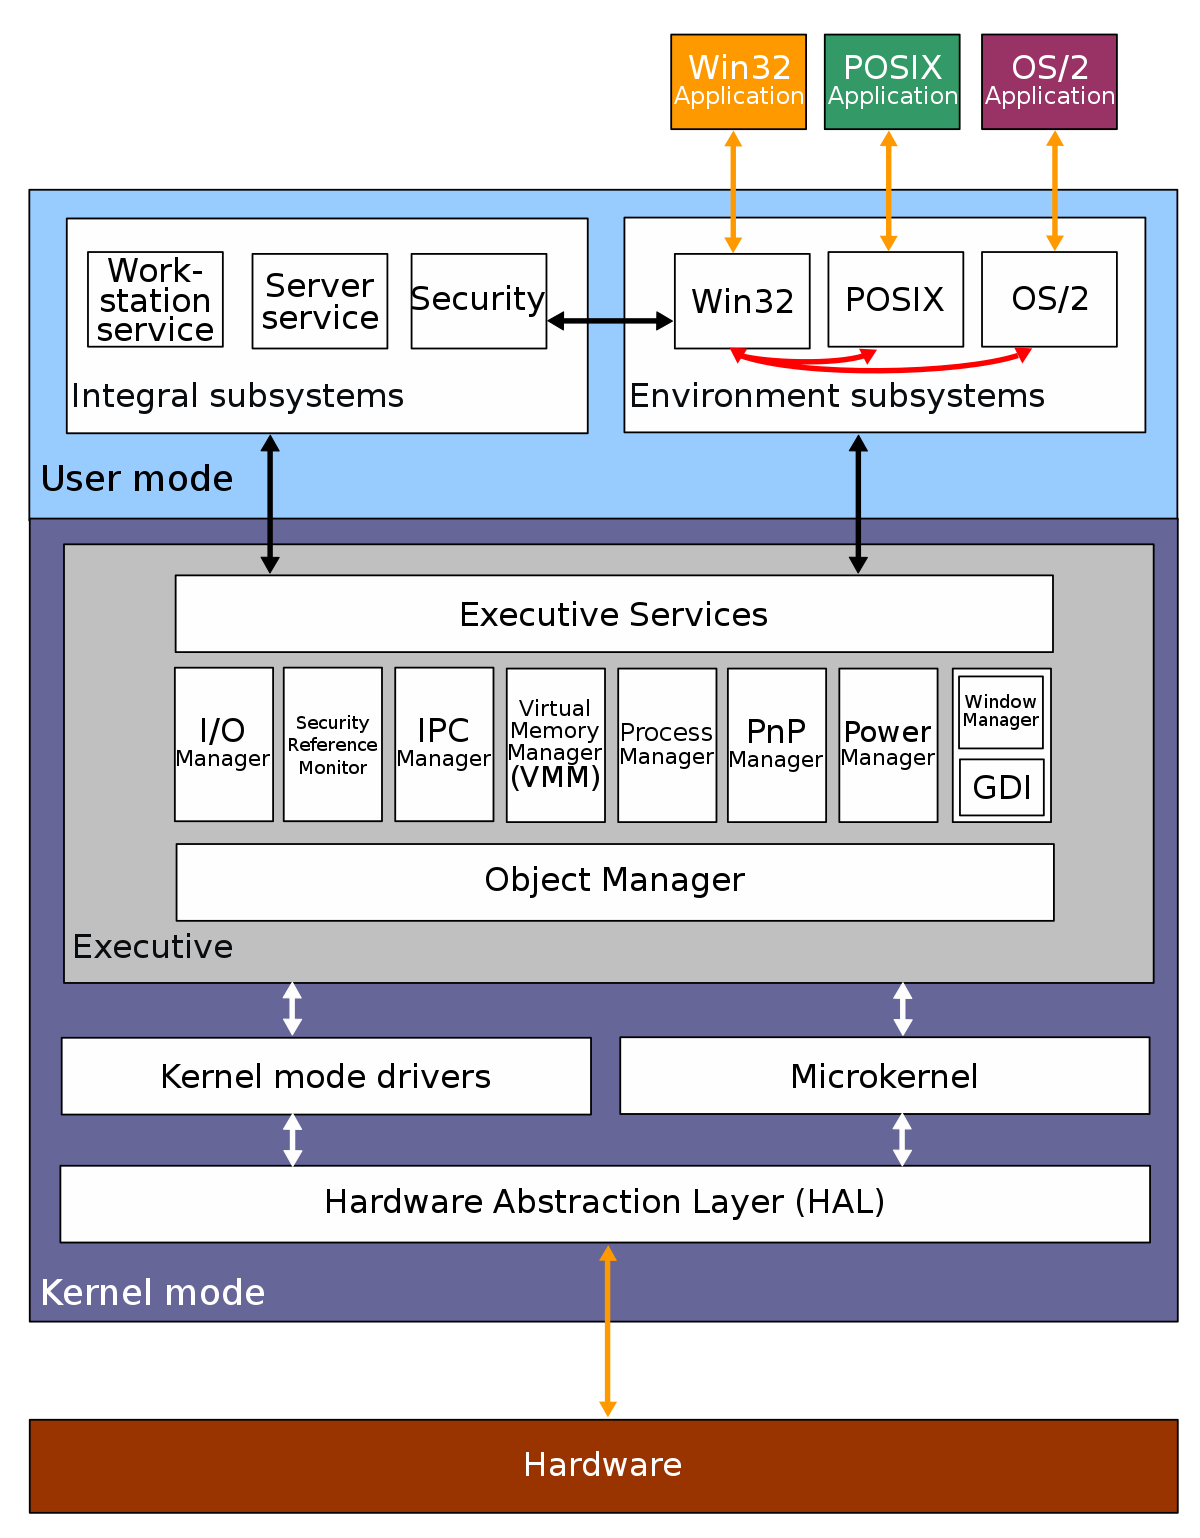
\includegraphics[width=0.8\textwidth]{../../images/microkernel0}
            \end{center}
        \end{column}
        \begin{column}{0.5\textwidth}
            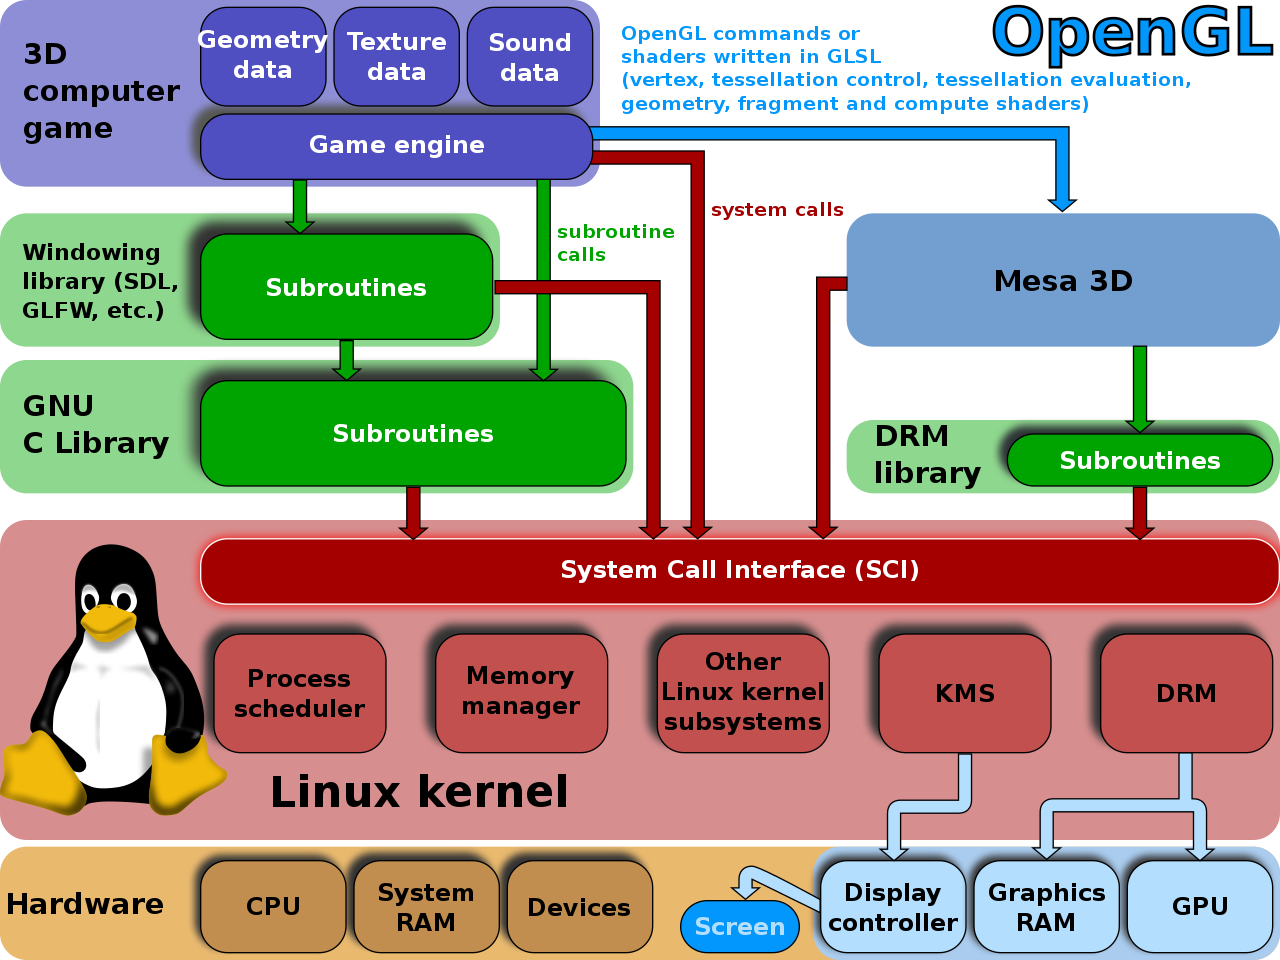
\includegraphics[width=\textwidth]{../../images/microkernel1}
        \end{column}
    \end{columns}
\end{frame}

    \begin{frame}{Arsitektur Plugin}
        \vspace{30pt}
        \centering
        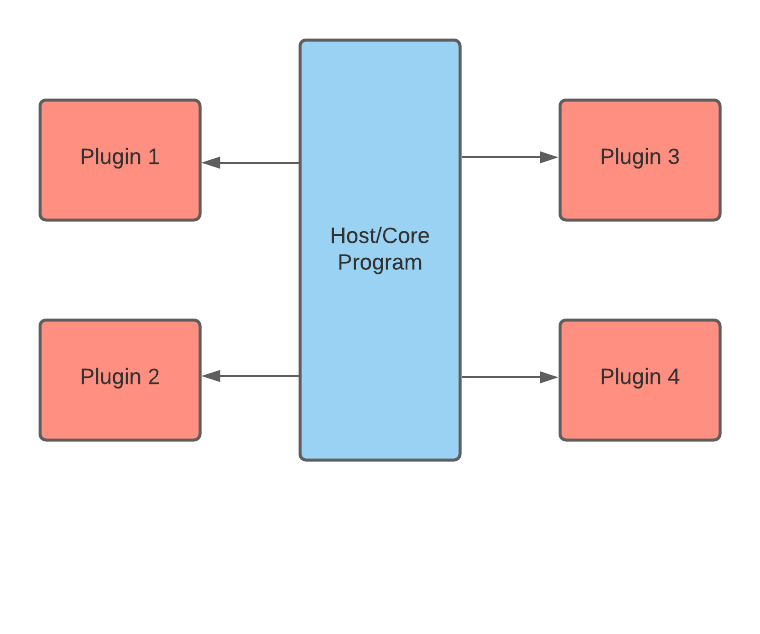
\includegraphics[width=0.7\textwidth]{../../images/plugin2}
    \end{frame}


    % Slide 4: Proses
    \begin{frame}{Proses}
        \begin{itemize}
            \item Komunikasi antara mikrokernel dan plugin biasanya dicapai melalui pengiriman pesan atau panggilan fungsi.
            \item Plugin dapat mendaftarkan diri dengan mikrokernel dan berkomunikasi satu sama lain menggunakan antarmuka yang terdefinisi dengan baik.
        \end{itemize}
    \end{frame}

    % Slide 5: Keuntungan
    \begin{frame}{Keuntungan}
        \begin{itemize}
            \item \textbf{Modularitas}: Arsitektur Microkernel/Plugin mempromosikan modularitas dengan memungkinkan komponen-komponen sistem dikembangkan dan dipelihara secara independen.
            \item \textbf{Extensibilitas}: Fungsionalitas baru dapat ditambahkan ke sistem tanpa memodifikasi mikrokernel inti.
            \item \textbf{Fleksibilitas}: Sistem dapat disesuaikan dengan memuat plugin-plugin tertentu pada waktu eksekusi.
        \end{itemize}
    \end{frame}

    % Slide 6: Kerugian
    \begin{frame}{Kerugian}
        \begin{itemize}
            \item \textbf{Beban Kinerja}: Komunikasi antara mikrokernel dan plugin dapat memperkenalkan beban kinerja dibandingkan dengan arsitektur monolitik.
            \item \textbf{Kompleksitas}: Mengelola interaksi antara mikrokernel dan plugin dapat menjadi kompleks, terutama dalam sistem berskala besar.
            \item \textbf{Dukungan Perangkat Keras Terbatas}: Beberapa fungsionalitas perangkat keras mungkin sulit diimplementasikan sebagai plugin, menyebabkan dukungan perangkat keras terbatas.
        \end{itemize}
    \end{frame}

    % Slide 7: Contoh
    \begin{frame}{Contoh}
        \begin{itemize}
            \item MINIX: MINIX adalah sistem operasi berbasis mikrokernel yang dikenal karena kesederhanaan dan modularitasnya. Ia menggunakan arsitektur mikrokernel dengan driver perangkat dan sistem file yang diimplementasikan sebagai plugin.
            \item Eclipse: Eclipse adalah lingkungan pengembangan terpadu (IDE) yang mengikuti arsitektur berbasis plugin. Pengembang dapat memperluas fungsionalitas Eclipse dengan menginstal plugin untuk berbagai bahasa pemrograman, kerangka kerja, dan alat.
        \end{itemize}
    \end{frame}

    \begin{frame}{Mikrokernel di Minix}
        \vspace{20pt}
        \centering
        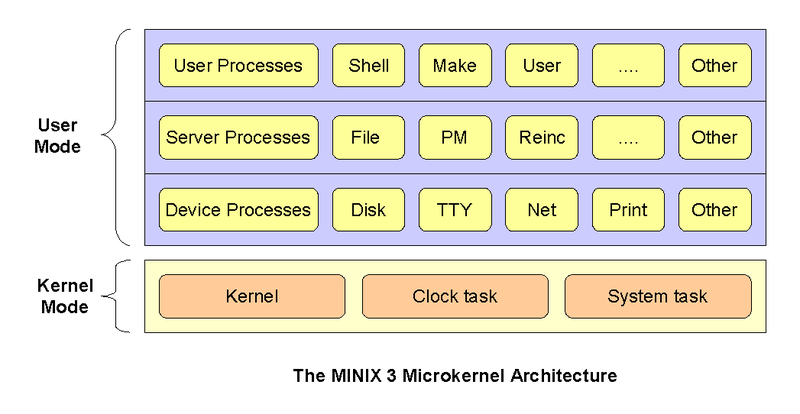
\includegraphics[width=\textwidth]{../../images/microkernel2}
    \end{frame}

    \begin{frame}{Arsitektur Plugin di Eclipse IDE}
        \vspace{10pt}
        \centering
        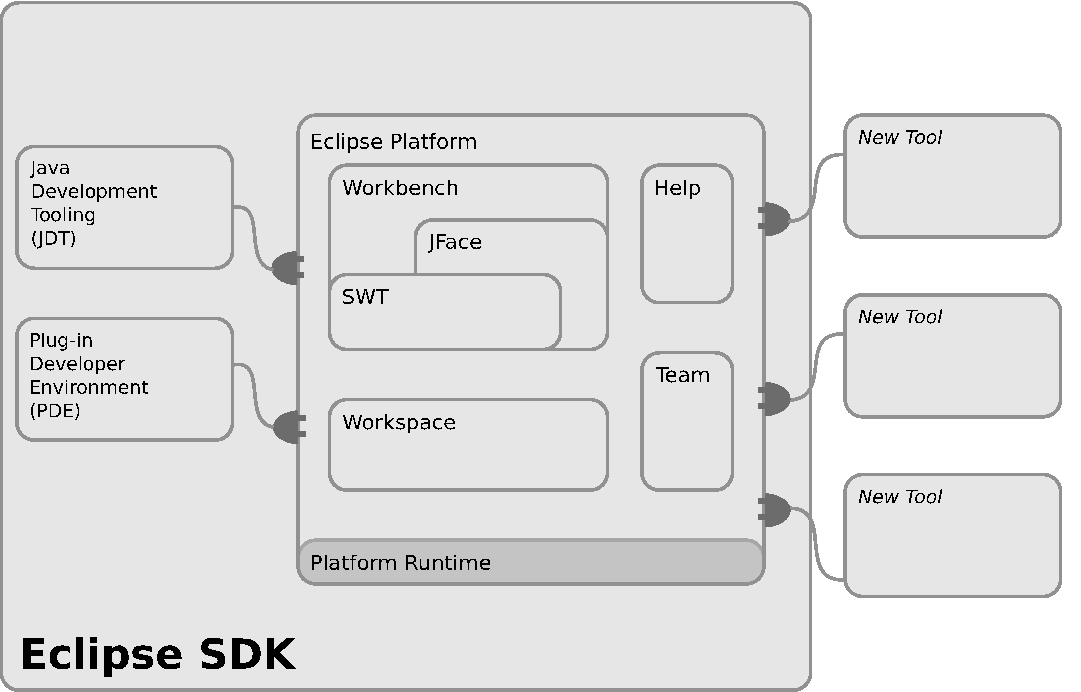
\includegraphics[width=0.78\textwidth]{../../images/plugin1}
    \end{frame}

    % Slide 8: Kesimpulan
    \begin{frame}{Kesimpulan}
        \begin{itemize}
            \item Arsitektur Microkernel/Plugin menawarkan pendekatan modular dan fleksibel untuk desain perangkat lunak, memungkinkan pengembangan sistem yang dapat disesuaikan dan diperluas.
            \item Meskipun memiliki keuntungan seperti modularitas dan extensibilitas, ia juga memiliki kelemahan seperti beban kinerja dan kompleksitas.
            \item Contoh-contoh dunia nyata seperti MINIX dan Eclipse menunjukkan aplikasi praktis dan manfaat Arsitektur Microkernel/Plugin dalam sistem perangkat lunak.
        \end{itemize}
    \end{frame}

\end{document}

